%%-----------------Chapter 6---------------------------
\chapter{Applying the Framework}\label{chap:results}

\section{Initial Automata Models}
\label{sec:results}
\subsection{Organism Automata}

Finding the general solution of $S \cdot v = 0$ is the first step in constructing the individual automata for Organism 1 and Organism 2 (as defined in section V - A ``Formulation of a Reference Model"). For Organism 1, directly solving $S \cdot v = 0$ renders the basis vectors $b_1 = [1, 0, 0.1, 1, -1, -1, 1, 0]$, $b_2 = [0, 1, -0.2, -3, 0, 3, -3, 2]$. However, these must be modified slightly before they can be directly used in constructing an automaton - since $v$ (with respect to Organism 1) has the form $[R_1, R_2, R_3, R_4, J_1, J_2, J_3, J_4]$ and reactions are taken to be irreversible (with reversible reactions split into pairs of irreversible reactions), each internal reaction $R_x$, $1 \leq x \leq 4$ should have positive flux.

Thus, the $b_2$ vector must be modified such that the character of the vector as a structural element of the flux cone is preserved, but each internal flux is made positive. Since multiplying $b_2$ by a negative scalar does not help ($R_2$ becomes negative), the only other operation that can be performed on $b_2$ that keeps the resultant vector within the flux cone is the addition of a scalar multiple of $b_1$ to $b_2$. Specifically, the minimal (magnitude) scalar $m_{min}$ must be found whereby $b_2^* = b_1 * m_{min} + b_2$ obeys $R_x \geq 0$, $1 \leq x \leq 4$. $m_{min}$ is trivially found to be 3 and the resulting $b_2^* = [3, 1, 0.1, 0, -3, 0, 0, 2]$ is used to replace $b_2$ within $B$.

While the previous process is performed in an \textit{ad hoc} fashion, the concepts involved (constraining the solution of $S \cdot v = 0$ such that internal fluxes remain positive) are formalized by the theory of extreme pathways, which themselves comprise convex bases that span the flux cone. Since manually examining and modifying bases while ensuring that the flux cone remains structurally sound becomes intractable for any $|B| > 2$, the extreme pathways $X = \{ x_1, x_2, ..., x_n \}$ are preferred to the naive bases for any model more complex than Chiu's toy model. Indeed, the set $B = \{ b_1, b_2^* \}$ can be analytically justified in its usage by observing that the minimal pathways they represent directly correspond to the two basic metabolic pathways present in Organism 1. The $b_1$ vector represents the pathway that consumes $A_{env}$ and $C_{env}$ by means of $J_1$ and $J_2$ and produces $Y_{env}$ through $J_{3}$. This is known to be the preferred pathway for the organism. The $b_2^*$ vector represents the pathway that consumes $A_{env}$ by means of $J_1$ and produces $W_{env}$ through $J_4$ as a metabolite. This alternative pathway is taken when $C_{env}$ is absent. It is also observable that this pathway is less efficient -- it consumes three $A_{env}$ for the same amount of biomass accumulation (through $R_3$) that consuming one $A_{env}$ and one $C_{env}$ results in. Thus, given the \textit{a posteriori} knowledge of how Organism 1 should function, the usage of $B$ suffices for all practical purposes.


Solving $S \cdot v = 0$ for Organism 2 is a simpler case, rendering $B = \{ [1, 0.02, -1, -1, 1] \}$, which needs no further modification as $R_5$ and $R_6$ are both positive. In the same analytic process as was performed for Organism 1, the $b_1$ vector has a clear metabolic interpretation -- a single pathway exists that consumes $A_{env}$ and $B_{env}$ through $J_5$ and $J_6$, respectively, and produces $C_{env}$ by means of $J_7$. This is expected and consistent with known behavior of Organism 2. Thus, each location in the automata models of Organism 1/2 represents a distinct metabolic state, as shown in Fig \ref{Organism1Automata} and Fig \ref{Organism2Automata}.

The bases as previously given, together with the full stoichiometry (internal as well as uptake/secretion) of each organism are transformed into hybrid automata by means of the Algorithm 2 procedure. Biomass accumulation and proper flux bounding are then added, according to the stoichiometry and bounds of each organism. While the $\overline{Q}$ variables should, in theory, be fully inclusive on the flux values such that it realizes $v_i * \Delta t$ upon $l_n \Rightarrow l_1$, $\overline{Q}$ has been restricted to the fluxes that are relevant for enforcing bounds (the uptake reactions) or accumulating biomass. This has been done to declutter the automata diagrams by removing superfluous equations as well as making the simulations significantly more efficient. Each additional variable has a multiplicative effect on the size of the reachable set -- the solver is not intelligent enough to determine that a point in the state space is the ``same" as its neighbor that only varies in one (superfluous) variable, so redundant work is done when exploring.

\begin{figure}[H]
\centering
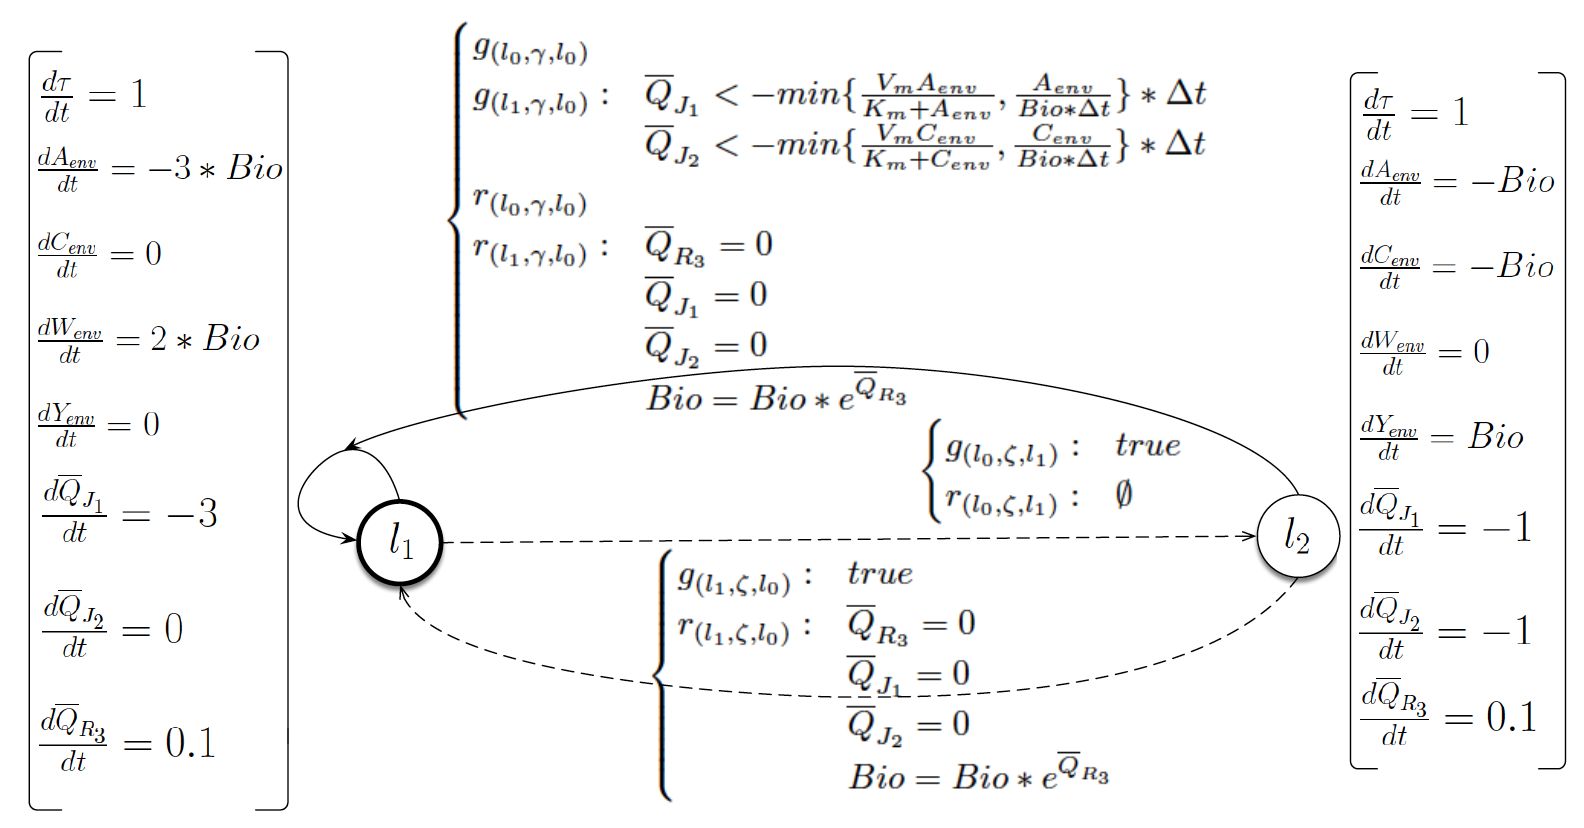
\includegraphics[width=1.0\textwidth]{figures/RedOrganismNoControl.png}
\caption{Automata representation of Organism 1}
\label{Organism1Automata}
\end{figure}

\begin{figure}[H]
\centering
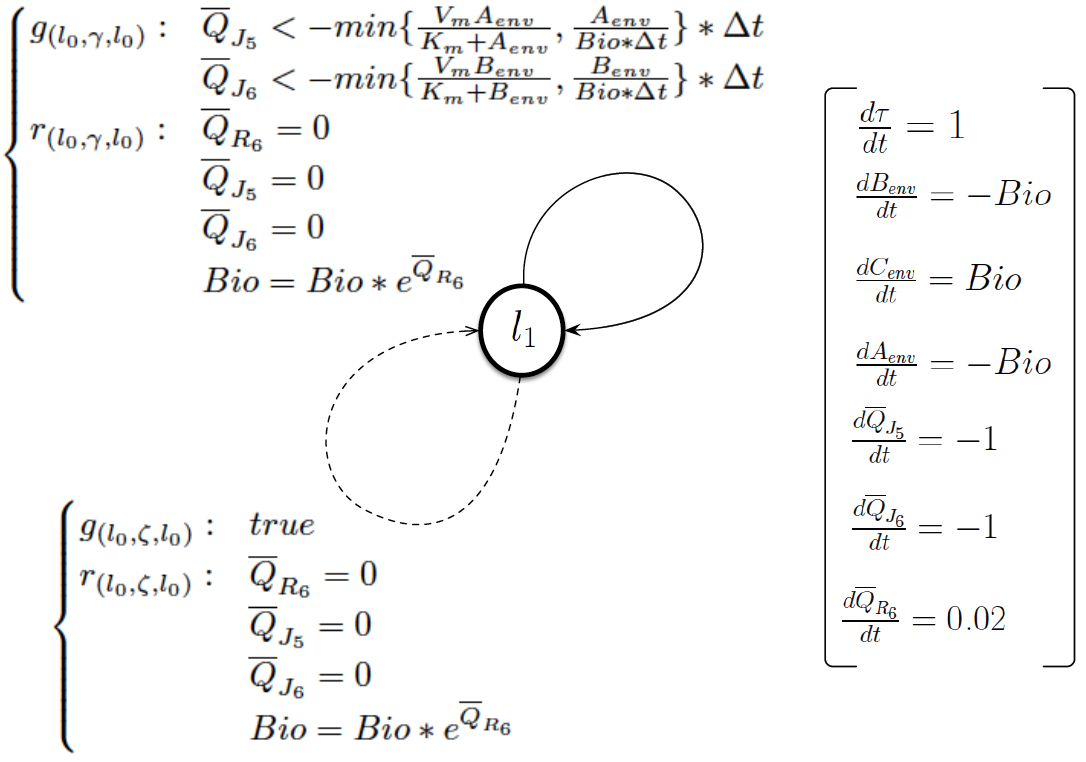
\includegraphics[width=1.0\textwidth]{figures/BlueOrganismNoControl.png}
\caption{Automata representation of Organism 2}
\label{Organism2Automata}
\end{figure}

\subsection{Deterministic Control of Model Organisms}

For Organism 1 (Fig \ref{Organism1ControlAutomata}), the control mechanism is known and can be used to replace the non-deterministic transitions between $l_1$ and $l_2$. The transition from $l_1$ to $l_2$ should be forced when the concentration of $C_{env}$, the metabolite that activates the preferred pathway, rises above some detection threshold $\epsilon$. The transition from $l_2$ back to $l_1$ should be forced when the concentration falls back below the threshold (as a result of uptake). The automata corresponding to Organism 2 (Fig \ref{Organism2ControlAutomata}) only has one location, so the non-determinism can be removed entirely. The deterministic transition, while somewhat superfluous, is necessary to ensure that the biomass is adequately updated.

\begin{figure}[H]
\centering
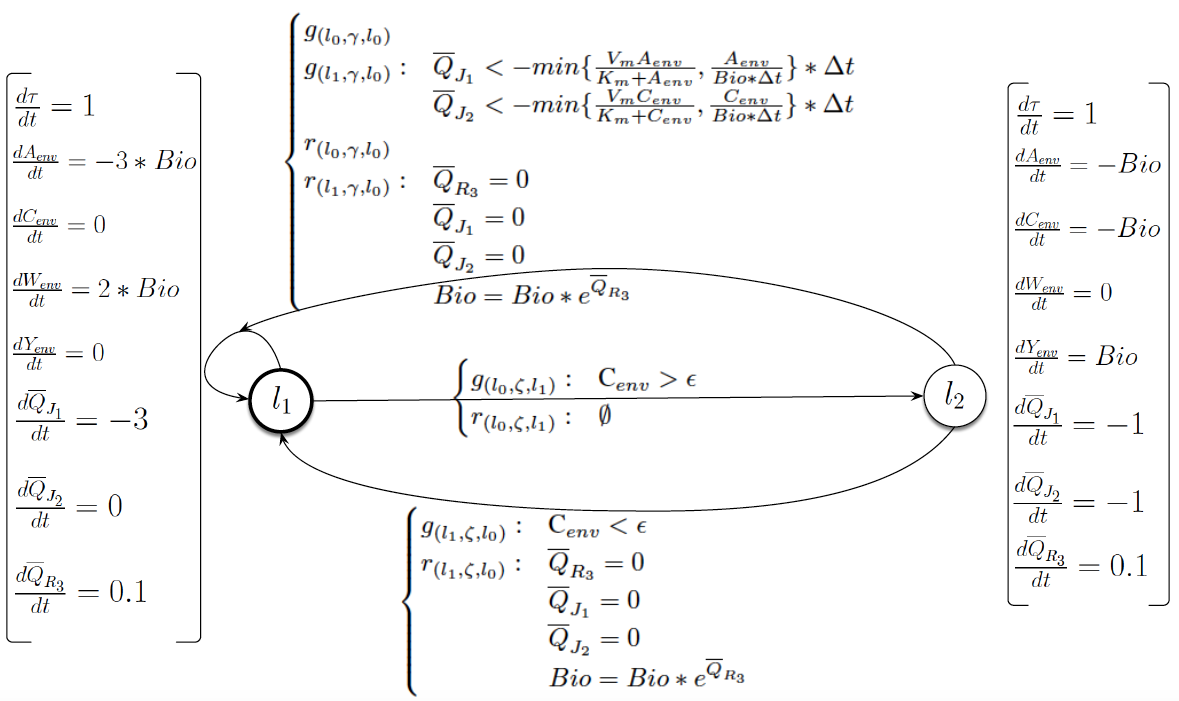
\includegraphics[width=1.0\textwidth]{figures/RedOrganismWithControl.png}
\caption{Organism 1 with Control Mechanism}
\label{Organism1ControlAutomata}
\end{figure}

\begin{figure}[H]
\centering
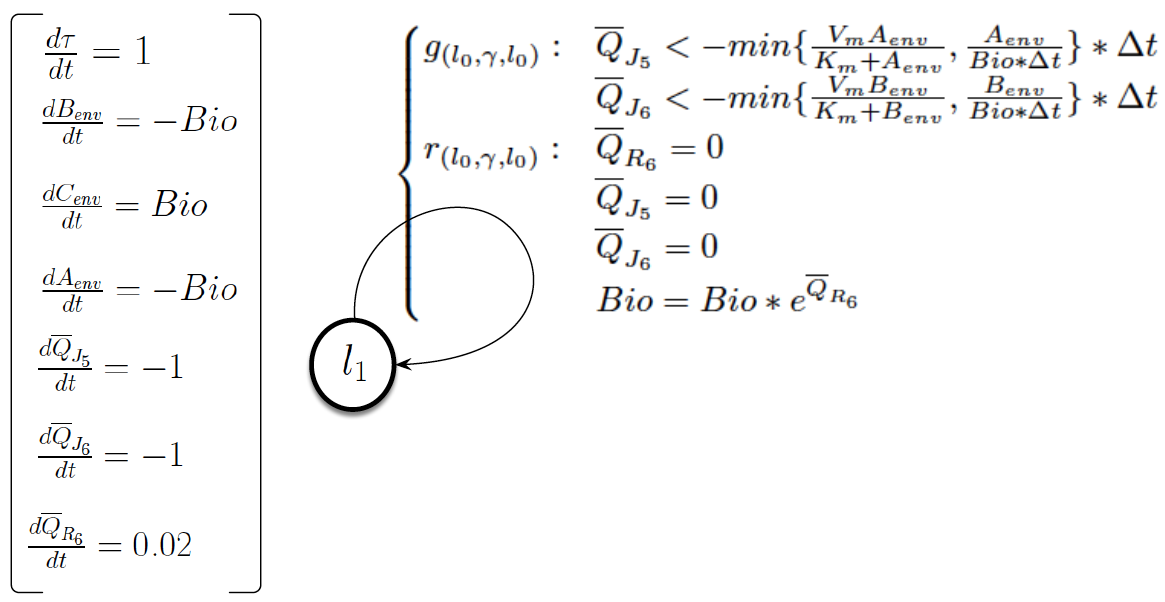
\includegraphics[width=1.0\textwidth]{figures/BlueOrganismWithControl.png}
\caption{Organism 2 with Control Mechanism}
\label{Organism2ControlAutomata}
\end{figure}


% insert organism 1 and 2 diagrams with control
%Given dFBA descriptions of Organism 1 as $\mathbb{D}_1$ and Organism 2 as $\mathbb{D}_2$, the transformation procedure of Algorithm 2 can be applied to receive $\mathbb{H}(\mathbb{D}_1)$ and $\mathbb{H}(\mathbb{D}_2)$. Note how the automaton corresponding to Organism 1 has two discrete states, while the automata corresponding to Organism 2 only has one discrete state. These directly correspond to the number of bases received when solving the system $S v = 0$ for $\mathbb{D}_1$ and $\mathbb{D}_2$. In Organism 2 in particular, a control mechanism of any variety is not necessary, because of the existence of a singular state. The transition back from the state, $S_1$, to itself, is only forced under one condition -- the bound, $v_{max}$ is violated by the accumulator vector. Any other transition taken from $S_1$ to itself is entirely nondeterministic. Further, the active dynamics of $\mathbb{H}(\mathbb{D}_2)$ never actually change; the accumulation and reset to $S_1$ is necessary, however, to ensure proper dFBA representation. This is particularly important when applying inner composition to form $\mathbb{H}(\mathbb{D}_1, \mathbb{D}_2)$ -- the synchronization of "reset" events is necessary to keep time-step size consistent.

%Whereas in Organism 2, the control mechanism from Chiu's work is directly applied -- when $C$ is present, choose the pathway that consumes $C$. Otherwise, choose the alternate pathway that only consumes $A$. The transitions associated with the control mechanism are clearly forced transitions, as is the transition associated with the $v_{max}$ boundary. The nondeterministic transitions so prevalent in the theoretical model are nowhere to be found, because they are largely used to under-specify a system when the control mechanism is unknown.
\subsection{Co-Culture Automaton}

The inner composition operation can be applied to the prior two automata to construct a model of the co-culture. However, a small change needs to be made before that operation can be performed successfully -- the biomass accumulation variable $Bio$ (not formally an internal metabolite) should be made distinct between the two organisms so the composition operation does not treat them as a common variable. Denote the two new variables $Bio_1$ and $Bio_2$ and update the resets accordingly. No further preprocessing is needed as the dynamics of $\overline{C}_{ext}$ will be properly combined and the $\overline{Q}$ variables are disjoint between the organisms.

\begin{figure}[H]
\centering
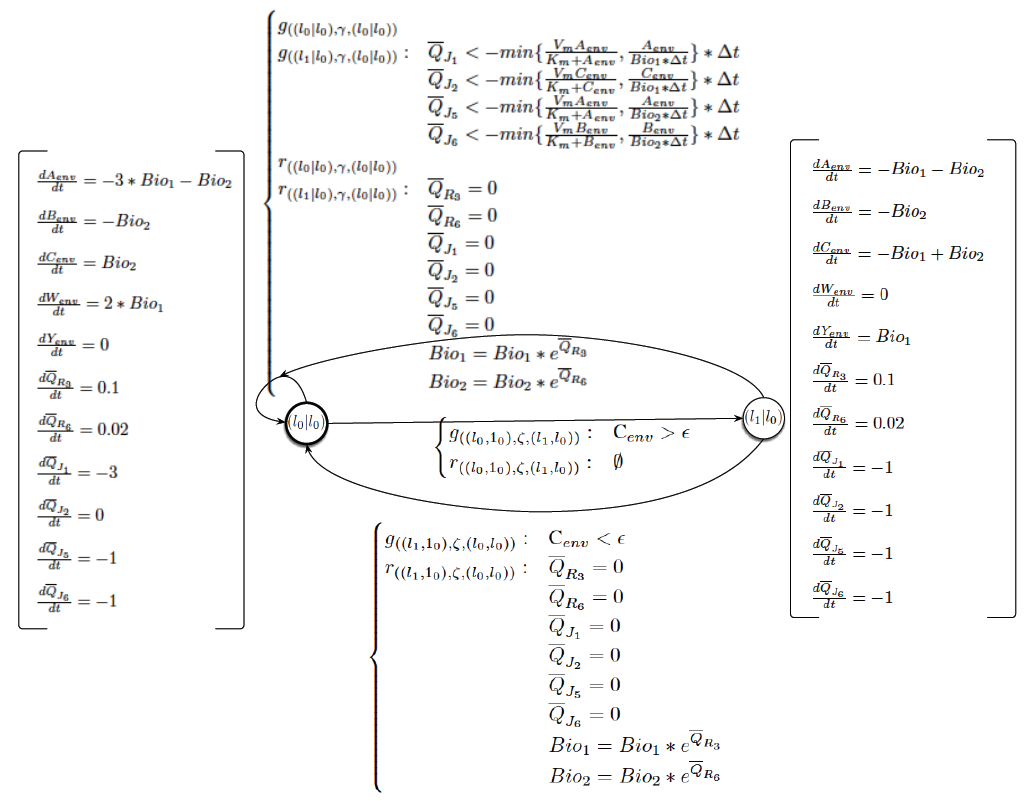
\includegraphics[width=1.0\textwidth]{figures/CoCultureWithControl.png}
\caption{Co-Culture with Control Mechanism}
\label{Organism3Automata}
\end{figure}

\section{Simulation Environment Setup}

\subsection{Automata Implementation in Ariadne}

\subsection{Automata Variations}

\subsection{Simulation Parameters}

\subsection{Simulation Output, Data Gathering, and Plotting}

\section{Experimental Results}

\subsection{Reachable Set Computation}

\subsection{Qualitative Behavior}

Upon formulating the previous three models using the libraries \textit{Ariadne} provides, a comparable simulation (Fig. \ref{SimResult}) to the one in Chiu's work was run to generate experimental results. We use the time scale $t_{max} = 20$ with $\Delta t = 0.01$. The automata under consideration are entirely deterministic, so only one run is necessary for each (no averaging of results is necessary).

\begin{figure}[H]
\centering
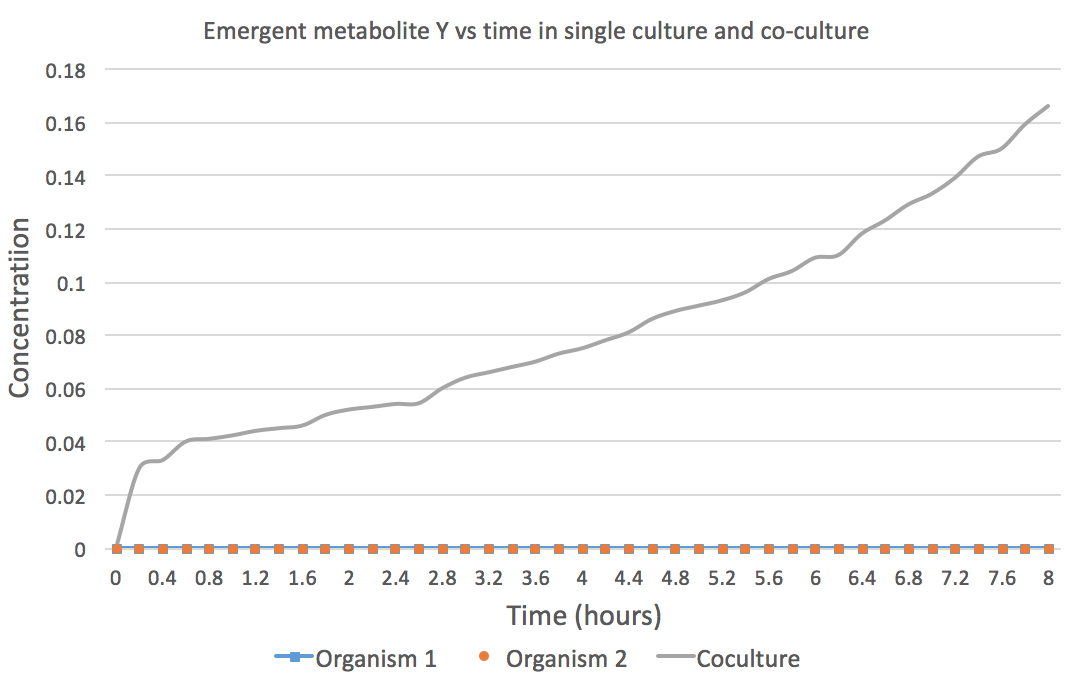
\includegraphics[width=1.0\textwidth]{figures/metabolite_concentration.png}
\caption{Levels of emergent metabolite Y in single cultures and co-culture}
\label{SimResult}
\end{figure}

\subsection{Formal Verification of Emergent Metabolism}